\documentclass[border=0.5mm]{standalone}

\usepackage{import}
\subimport{../../../}{preamble.tex}

\usepackage{tikz}
\usetikzlibrary{calc}

% f(x) = (0.1 x_1^2 + 0.6 x_2^2)/2, L = 1, beta = (1-sqrt(0.1))/(1+sqrt(0.1))
% Iterates computed exactly; the contours are the level sets of f through the
% points where the gradient is evaluated, so each gradient step is orthogonal to them.
\tikzset{
  contour/.style={black!40},
  iterate/.style={circle, fill=black, inner sep=1.2pt},
  lookahead/.style={circle, fill=blue, inner sep=1.2pt},
  grad/.style={->, >=stealth, red, thick},
  mom/.style={->, >=stealth, blue, thick, dashed},
}

% Level sets {x : f(x) = c} for the levels c in #1
\newcommand{\contours}[1]{
  \begin{scope}
    \clip (-4.6,-0.7) rectangle (-1.4,2.3);
    \foreach \c in {#1} {
      \draw[contour] (0,0) ellipse ({sqrt(2*\c/0.1)} and {sqrt(2*\c/0.6)});
    }
  \end{scope}
}

% Right-angle mark at #1 between the gradient step towards #2 and the contour
\newcommand{\rightangle}[2]{
  \draw[black!60] ($(#1)!4pt!(#2)$) -- ($($(#1)!4pt!(#2)$)+($(#1)!4pt!90:(#2)$)-(#1)$) -- ($(#1)!4pt!90:(#2)$);
}

\begin{document}

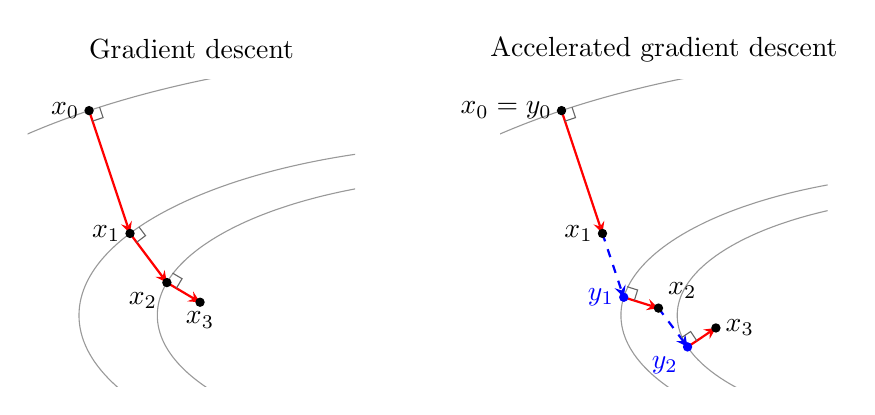
\begin{tikzpicture}[x=1.3cm, y=1.3cm]

  % Gradient descent
  \begin{scope}
    \contours{2, 0.84, 0.5556}
    \node at (-3, 2.6) {Gradient descent};
    \coordinate (x0) at (-4, 2);
    \coordinate (x1) at (-3.6, 0.8);
    \coordinate (x2) at (-3.24, 0.32);
    \coordinate (x3) at (-2.916, 0.128);
    \draw[grad] (x0) -- (x1);
    \draw[grad] (x1) -- (x2);
    \draw[grad] (x2) -- (x3);
    \rightangle{x0}{x1}
    \rightangle{x1}{x2}
    \rightangle{x2}{x3}
    \foreach \p in {x0, x1, x2, x3} { \node[iterate] at (\p) {}; }
    \node[left] at (x0) {$x_0$};
    \node[left] at (x1) {$x_1$};
    \node[below left] at (x2) {$x_2$};
    \node[below] at (x3) {$x_3$};
  \end{scope}

  % Accelerated gradient descent
  \begin{scope}[xshift=6cm]
    \contours{2, 0.5847, 0.4118}
    \node at (-3, 2.6) {Accelerated gradient descent};
    \coordinate (x0) at (-4, 2);
    \coordinate (x1) at (-3.6, 0.8);
    \coordinate (y1) at (-3.3922, 0.1766);
    \coordinate (x2) at (-3.0530, 0.0706);
    \coordinate (y2) at (-2.7688, -0.3083);
    \coordinate (x3) at (-2.4919, -0.1233);
    \draw[grad] (x0) -- (x1);
    \draw[mom] (x1) -- (y1);
    \draw[grad] (y1) -- (x2);
    \draw[mom] (x2) -- (y2);
    \draw[grad] (y2) -- (x3);
    \rightangle{x0}{x1}
    \rightangle{y1}{x2}
    \rightangle{y2}{x3}
    \foreach \p in {x0, x1, x2, x3} { \node[iterate] at (\p) {}; }
    \foreach \p in {y1, y2} { \node[lookahead] at (\p) {}; }
    \node[left] at (x0) {$x_0=y_0$};
    \node[left] at (x1) {$x_1$};
    \node[left, blue] at (y1) {$y_1$};
    \node[above right] at (x2) {$x_2$};
    \node[below left, blue] at (y2) {$y_2$};
    \node[right] at (x3) {$x_3$};
  \end{scope}

\end{tikzpicture}

\end{document}

%%% Local Variables:
%%% mode: latex
%%% TeX-master: t
%%% End:
